% *********************************************************************
% © 2021–2024 Jeremy Sylvestre
%
% Permission is granted to copy, distribute and/or modify this document
% under the terms of the GNU Free Documentation License, Version 1.3 or
% any later version published by the Free Software Foundation; with no
% Invariant Sections, no Front-Cover Texts, and no Back-Cover Texts. A
% copy of the license is included in the appendix entitled “GNU Free
% Documentation License” that appears in the output document of this
% PreTeXt source code. All trademarks™ are the registered® marks of
% their respective owners.
%
% *********************************************************************

\newcommand*{\xmin}{-2}
\newcommand*{\xmax}{2.5}
\newcommand*{\ymin}{-1}
\newcommand*{\ymax}{4.5}

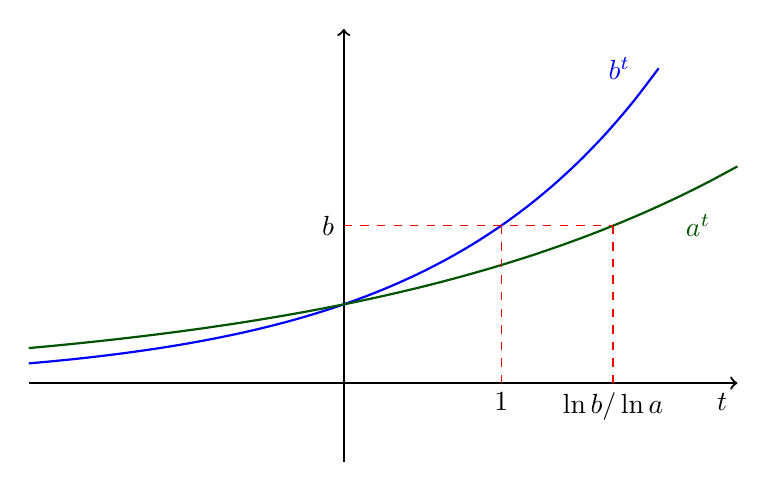
\begin{tikzpicture}
[
	closedpt/.style={circle,draw,fill,inner sep=0pt,minimum size=4pt},
	openpt/.style={circle,draw,inner sep=0pt,minimum size=4pt},
	xscale=2
]

	% axes
	\draw[->,thick] (\xmin,0) -- (\xmax,0) node[below left] {$t$};
	\draw[->,thick] (0,\ymin) -- (0,\ymax);

	\draw[blue,smooth,domain=-2:2,thick] plot (\x, {exp (0.693 * \x)});
	\node[blue] at (1.75,4) {$b^t$};
	\draw[green!33!black,smooth,domain=-2:2.5,thick] plot (\x, {exp (0.405 * \x)});
	\node[green!33!black] at (2.25,2) {$a^t$};

	\draw[dashed,red]
	  (0,2)    -- (1,2) -- (1.71,2)
	  (1,2)    -- (1,0)
	  (1.71,2) -- (1.71,0)
	;
	\node[left] at (0,2) {$b$};
	\node[below] at (1,0) {$1$};
	\node[below] at (1.71,0) {$\ln b / \ln a$};

	% \node[red,closedpt] at (2,4) (pt) {};
	% \node[left,red] at (0,4) (y) {$b$};
	% \node[below,red] at (2,0) (t) {?};
	% \draw[red,dashed] (y) -- (pt) -- (t);

\end{tikzpicture}
